\documentclass[border=10pt,tikz]{standalone} 
\usepackage{verbatim}
\usepackage{tikz}
\begin{document}
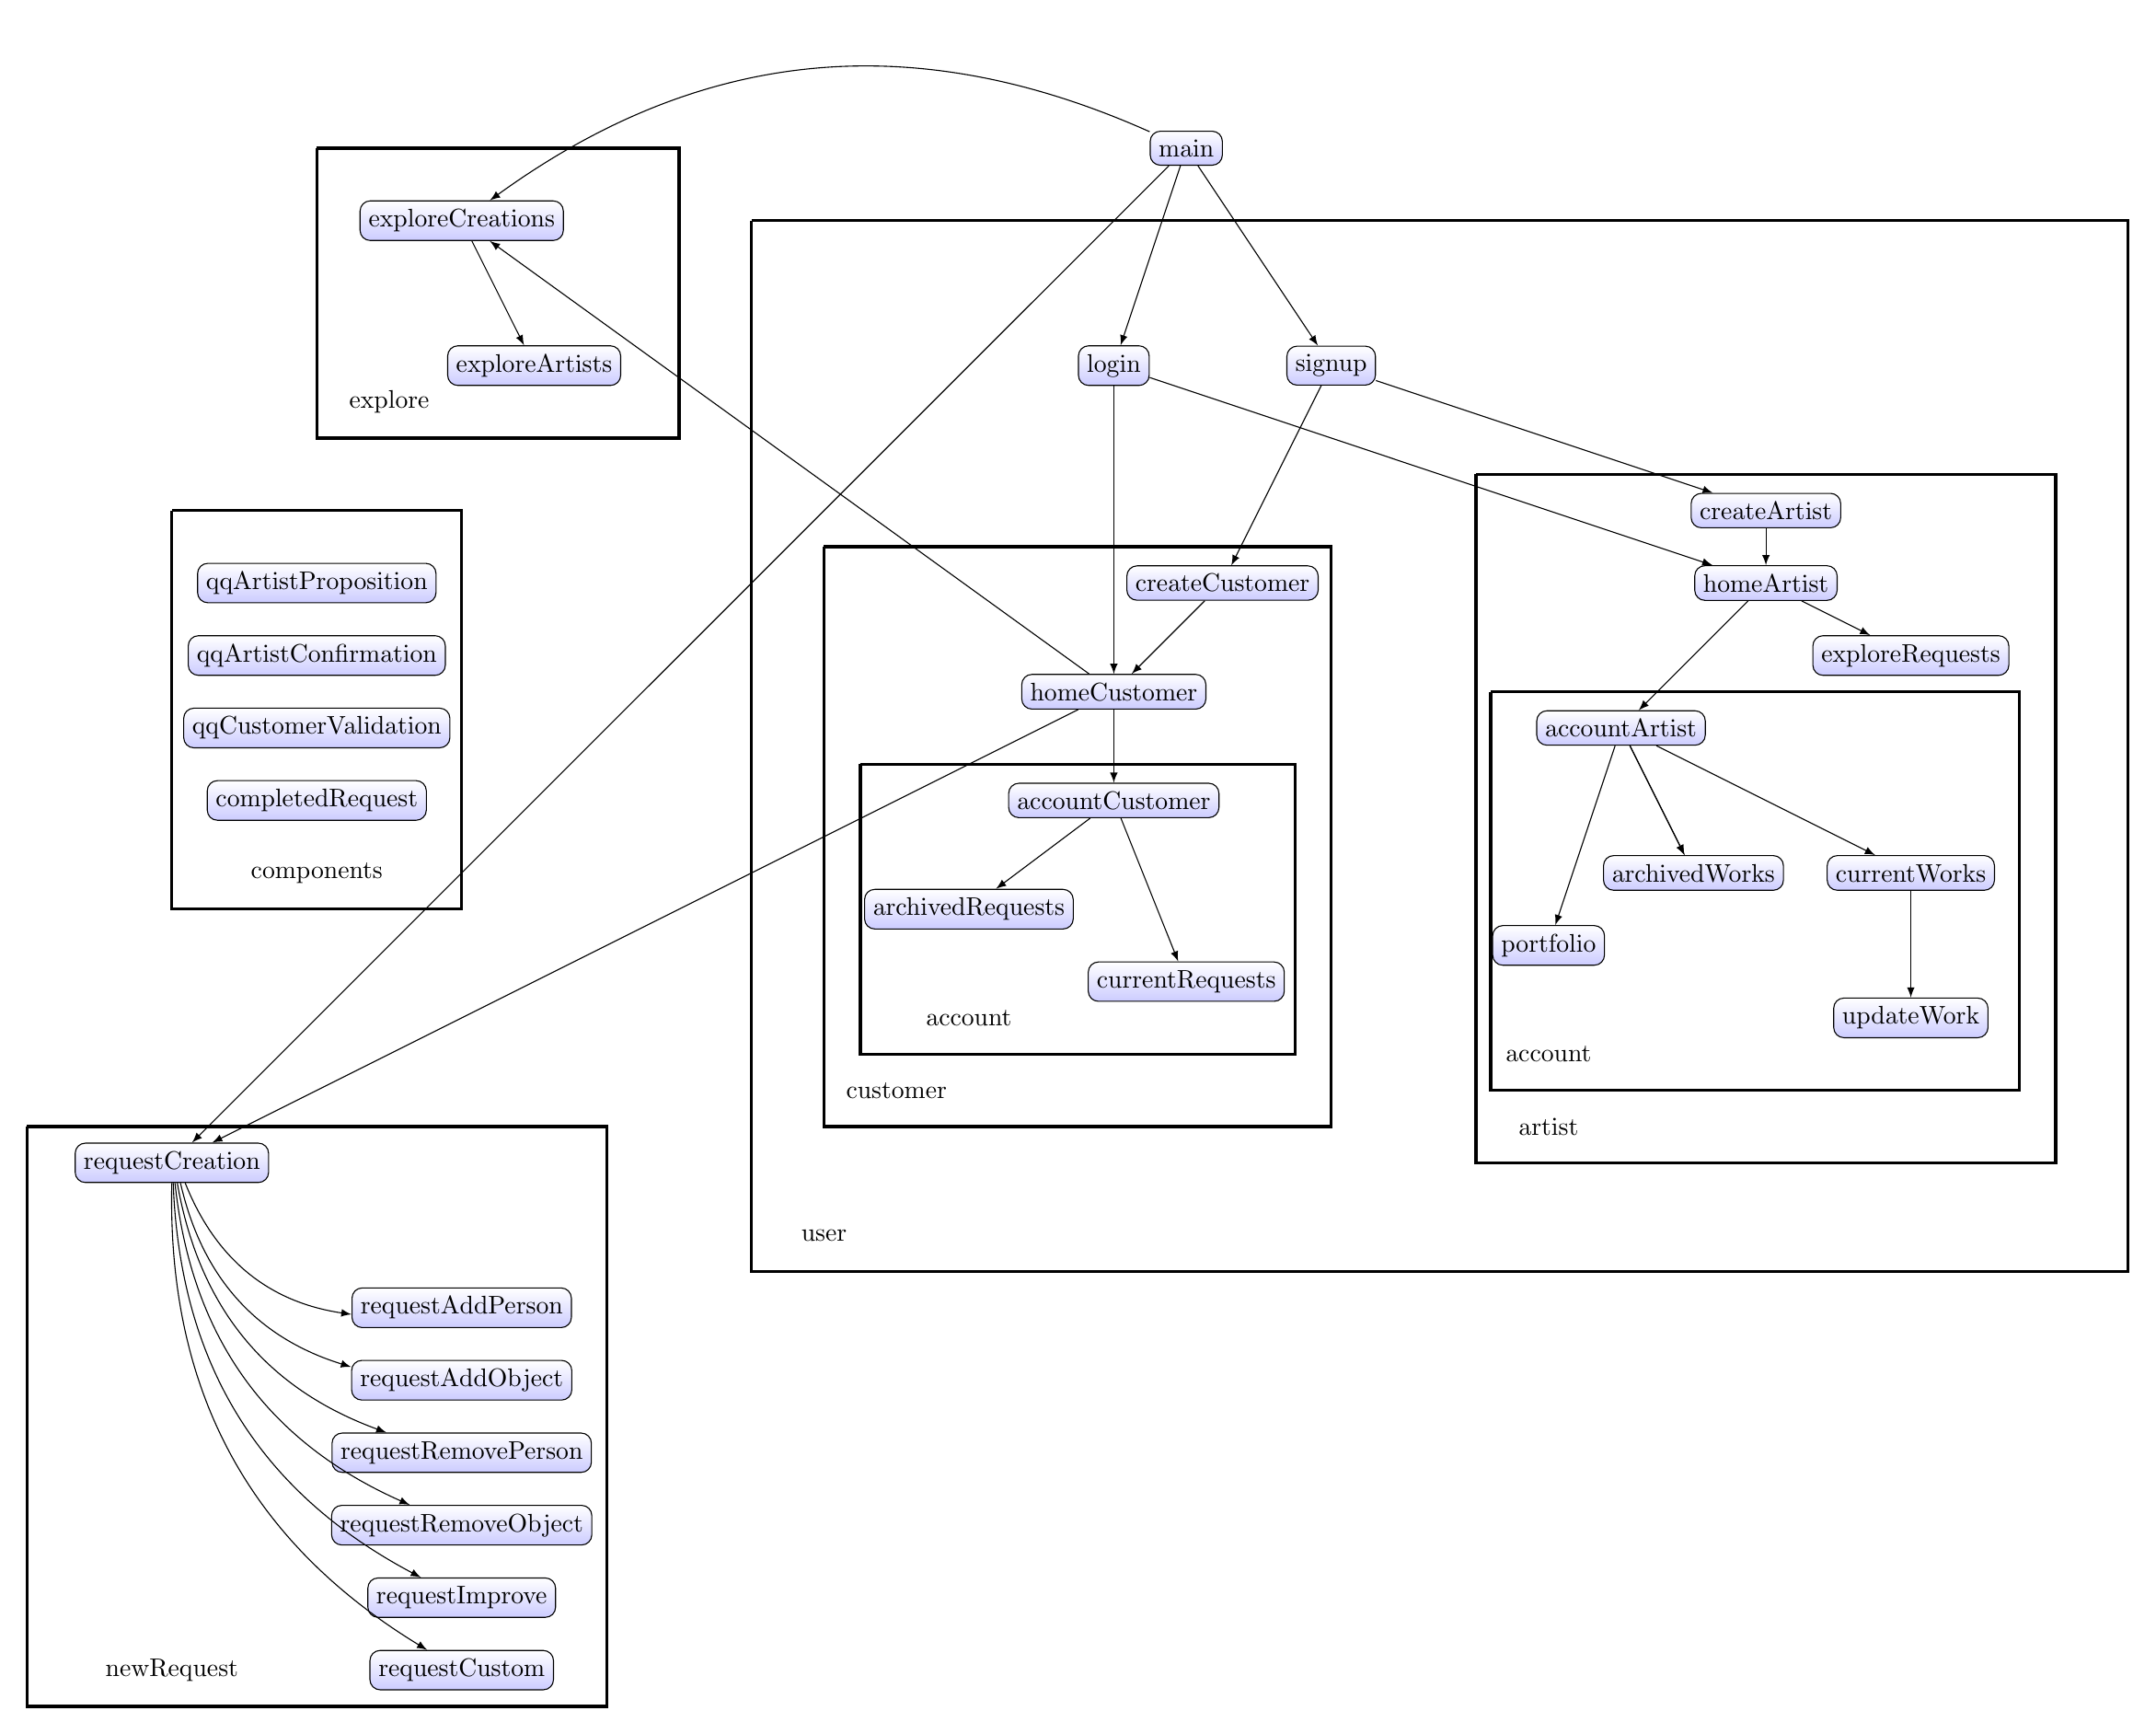
\begin{tikzpicture}

\tikzstyle{vertex}=[shape=rectangle, rounded corners,
    draw, align=center,
    top color=white, bottom color=blue!20]

  \node[vertex] (main) at (0,2) {main};

  \node[vertex] (login) at (-1,-1) {login};
  \node[vertex] (signup) at (2,-1) {signup};

  \draw[->,>=latex] (main) -- (signup);
  \draw[->,>=latex] (main) -- (login);

  \node[vertex] (createCustomer) at (0.5,-4) {createCustomer};
  \node[vertex] (createArtist) at (8,-3) {createArtist};

  \draw[->,>=latex] (signup) -- (createCustomer);
  \draw[->,>=latex] (signup) -- (createArtist);

  \node[vertex] (homeCustomer) at (-1,-5.5) {homeCustomer};
  \node[vertex] (homeArtist) at (8,-4) {homeArtist};

  \draw[->,>=latex] (createCustomer) -- (homeCustomer);
  \draw[->,>=latex] (createArtist) -- (homeArtist);


  \draw[->,>=latex] (login) -- (homeCustomer);
  \draw[->,>=latex] (login) -- (homeArtist);

  \node[vertex] (requestCreation) at (-14,-12) {requestCreation};
  \node[vertex] (exploreCreations) at (-10,1) {exploreCreations};

  \node[vertex] (exploreArtists) at (-9,-1) {exploreArtists};
 \draw[->,>=latex] (exploreCreations) -- (exploreArtists);

  \draw[->,>=latex] (main) to (requestCreation);
  \draw[->,>=latex] (homeCustomer) -- (requestCreation);

  \draw[->,>=latex] (main) to[bend right] (exploreCreations);
  \draw[->,>=latex] (homeCustomer) -- (exploreCreations);


	\node[vertex] (requestAddPerson) at (-10,-14) {requestAddPerson};
	\node[vertex] (requestAddObject) at (-10,-15) {requestAddObject};
	\node[vertex] (requestRemovePerson) at (-10,-16) {requestRemovePerson};
	\node[vertex] (requestRemoveObject) at (-10,-17) {requestRemoveObject};
	\node[vertex] (requestImprove) at (-10,-18) {requestImprove};
	\node[vertex] (requestCustom) at (-10,-19) {requestCustom};

	


 \draw[->,>=latex] (requestCreation) to[bend right]  (requestAddPerson);
 \draw[->,>=latex] (requestCreation)  to[bend right]  (requestAddObject);
 \draw[->,>=latex] (requestCreation)  to[bend right]  (requestRemovePerson);
 \draw[->,>=latex] (requestCreation)  to[bend right]  (requestRemoveObject);
\draw[->,>=latex] (requestCreation)  to[bend right]  (requestImprove);
\draw[->,>=latex] (requestCreation)  to[bend right]  (requestCustom);


\node[vertex] (exploreRequests) at (10,-5) {exploreRequests};
\draw[->,>=latex] (homeArtist) -- (exploreRequests);

\node[vertex] (accountCustomer) at (-1,-7) {accountCustomer};
\node[vertex] (accountArtist) at (6,-6) {accountArtist};

\node[vertex] (archivedRequests) at (-3,-8.5) {archivedRequests};
\node[vertex] (currentRequests) at (0,-9.5) {currentRequests};

\draw[->,>=latex] (accountCustomer) -- (archivedRequests);
\draw[->,>=latex] (accountCustomer) -- (currentRequests);


\node[vertex] (currentWorks) at (10, -8) {currentWorks};
\node[vertex] (archivedWorks) at (7, -8) {archivedWorks};

\draw[->,>=latex] (homeCustomer) -- (accountCustomer);
\draw[->,>=latex] (homeArtist) -- (accountArtist);
\draw[->,>=latex] (accountArtist) -- (currentWorks);
\draw[->,>=latex] (accountArtist) -- (archivedWorks);


\node[vertex] (updateWork) at  (10, -10)  {updateWork};
\draw[->,>=latex] (accountArtist) -- (archivedWorks);
\draw[->,>=latex] (currentWorks) -- (updateWork);



\node[vertex] (portfolio) at (5,-9) {portfolio};
\draw[->,>=latex] (accountArtist) -- (portfolio);



% newRequest
\draw[very thick] (-16,-11.5) -- (-8,-11.5) -- (-8,-19.5) -- (-16,-19.5) -- (-16,-11.5);
\node (DOC_newRequest) at (-14,-19) {newRequest};


% artist
\draw[very thick] (4,-2.5) -- (12,-2.5) -- (12,-12) -- (4,-12) -- (4,-2.5);
\node (DOC_artist) at (5,-11.5) {artist};

% customer
\draw[very thick] (-5,-3.5) -- (2,-3.5) -- (2,-11.5) -- (-5,-11.5) -- (-5,-3.5);
\node (DOC_customer) at (-4,-11) {customer};


% user
\draw[very thick] (-6,1) -- (13,1) -- (13,-13.5) -- (-6,-13.5) -- (-6,1);
\node (DOC_user) at (-5,-13) {user};

%account1
\draw[very thick] (-4.5,-6.5) -- (1.5,-6.5) -- (1.5,-10.5) -- (-4.5,-10.5) -- (-4.5,-6.5);
\node (DOC_account1) at (-3,-10) {account};

%account2
\draw[very thick] (4.2,-5.5) -- (11.5,-5.5) -- (11.5,-11) -- (4.2,-11) -- (4.2,-5.5);
\node (DOC_account2) at (5,-10.5) {account};

% explore
\draw[very thick] (-12,2) -- (-7,2) -- (-7,-2) -- (-12,-2) -- (-12,2);
\node (DOC_explore) at (-11,-1.5) {explore};


% components
\node[vertex] (qqArtistProposition) at (-12,-4) {qqArtistProposition};
\node[vertex] (qqArtistConfirmation) at (-12,-5) {qqArtistConfirmation};
\node[vertex] (qqCustomerValidation) at (-12,-6) {qqCustomerValidation};
\node[vertex] (completedRequest) at (-12,-7) {completedRequest};

\draw[very thick] (-14,-3) -- (-10,-3) -- (-10,-8.5) -- (-14,-8.5) -- (-14,-3);
\node (DOC_explore) at (-12,-8) {components};



\end{tikzpicture}
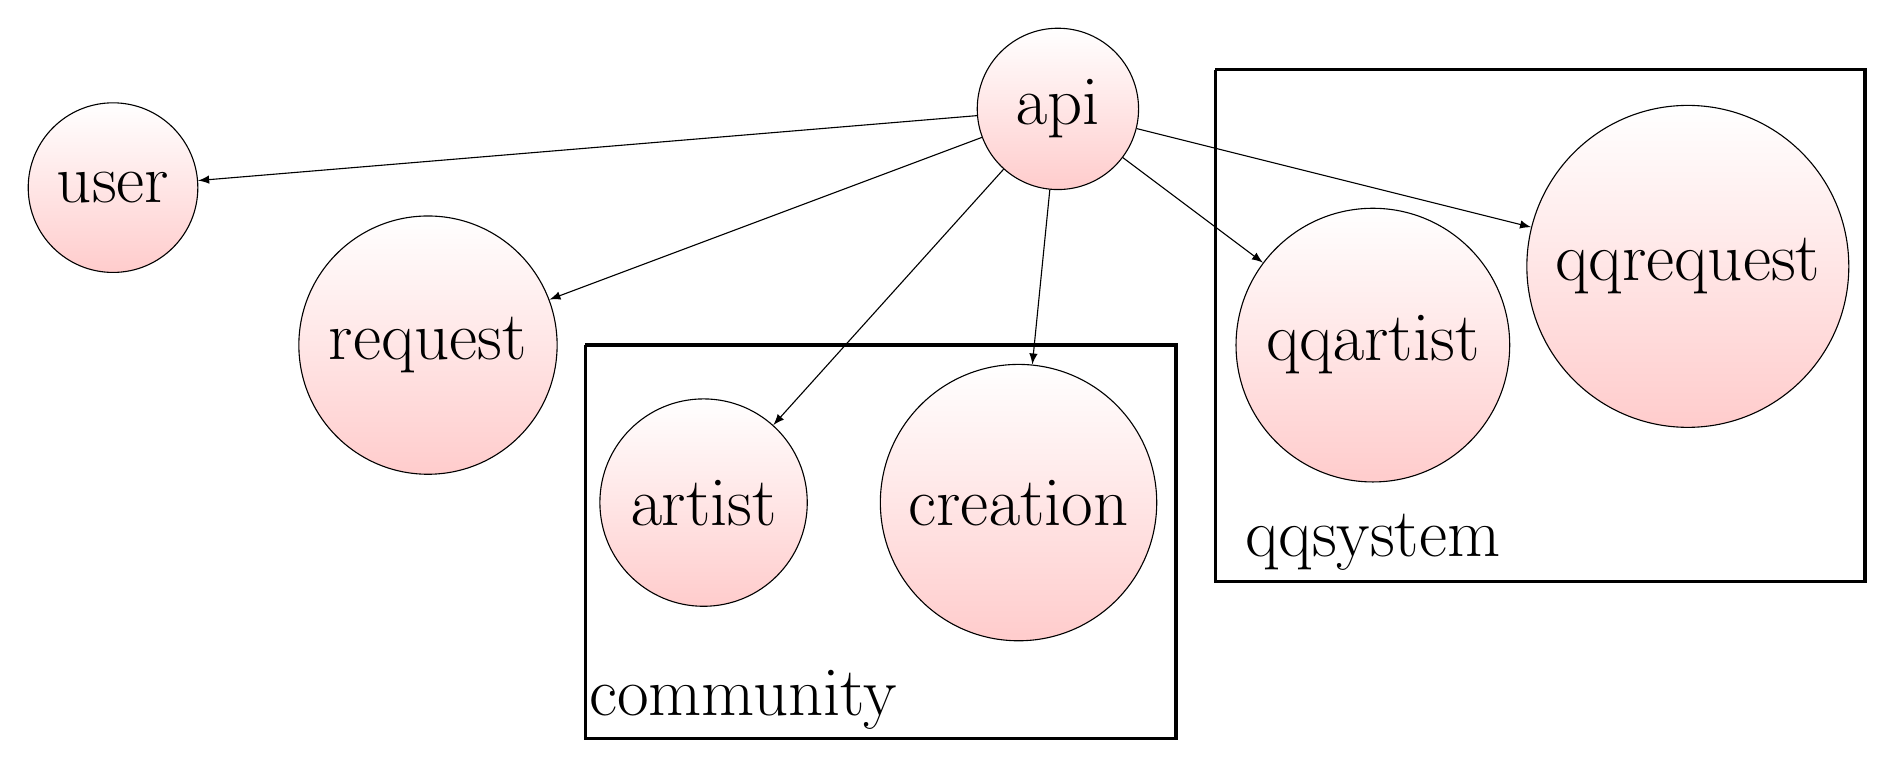
\begin{tikzpicture}


\tikzstyle{vertex}=[shape=circle, rounded corners,
    draw, align=center,
    top color=white, bottom color=red!20]
  \Huge
  \node[vertex] (api) at (0,0) {api};

  \node[vertex] (user) at (-12,-1) {user};
  \node[vertex] (request) at (-8,-3) {request};
  \node[vertex] (artist) at (-4.5,-5) {artist};
  \node[vertex] (creation) at (-0.5,-5) {creation};
  \node[vertex] (qqartist) at (4,-3) {qqartist};
  \node[vertex] (qqrequest) at (8,-2) {qqrequest};
  
  \draw[->,>=latex] (api) -- (user);
  \draw[->,>=latex] (api) -- (artist);
  \draw[->,>=latex] (api) -- (request);
  \draw[->,>=latex] (api) -- (creation);
  \draw[->,>=latex] (api) -- (qqartist);
  \draw[->,>=latex] (api) -- (qqrequest);
  
  % qqsystem
  \draw[very thick] (2,0.5) -- (10.25,0.5) -- (10.25,-6) -- (2,-6) -- (2,0.5);
  \node (DOC_explore) at (4,-5.5) {qqsystem};  
  % community
  \draw[very thick] (-6,-3) -- (1.5,-3) -- (1.5,-8) -- (-6,-8) -- (-6,-3);
  \node (DOC_explore) at (-4,-7.5) {community}; 


\end{tikzpicture}
\end{document}
